% =====================================================================
% BMED365: Computational Imaging
% Beamer Presentation - Topic List Y01-Y11
% =====================================================================
\documentclass[aspectratio=169, 10pt]{beamer}

% =====================================================================
% PACKAGES
% =====================================================================
\usepackage[utf8]{inputenc}
\usepackage[T1]{fontenc}
\usepackage[english]{babel}
\usepackage{graphicx}
\usepackage{tikz}
\usetikzlibrary{shapes.geometric, arrows, positioning, calc}
\usepackage{booktabs}
\usepackage{amsmath}
\usepackage{fontawesome5}
\usepackage{hyperref}
\hypersetup{colorlinks=true, linkcolor=blue, urlcolor=blue}

% =====================================================================
% THEME AND COLORS
% =====================================================================
\usetheme{Madrid}
\usecolortheme{seahorse}

% Custom colors
\definecolor{imagingcyan}{RGB}{0, 139, 139}
\setbeamercolor{structure}{fg=imagingcyan}

% =====================================================================
% TITLE INFO
% =====================================================================
\title{Computational Imaging}
\subtitle{BMED365: Topic List Y01--Y11}
\author{BMED365}
\date{Spring 2026}
\institute{Department of Biomedicine, University of Bergen}

% =====================================================================
% DOCUMENT
% =====================================================================
\begin{document}

% Title page
\begin{frame}
    \titlepage
\end{frame}

% Table of Contents
\begin{frame}{Overview}
    \tableofcontents
\end{frame}

% =====================================================================
% SECTION: Introduction to Computational Imaging
% =====================================================================
\section{Fundamentals of Computational Imaging}

\begin{frame}{Y01: Explain fundamental concepts in computational imaging}
    \textbf{What is Computational Imaging?}
    
    \vspace{0.3cm}
    \begin{block}{Definition}
        Computational imaging combines \textbf{optics}, \textbf{sensors}, and \textbf{algorithms} to create images that go beyond traditional photography -- extracting information invisible to conventional cameras.
    \end{block}
    
    \vspace{0.3cm}
    \begin{columns}[T]
        \begin{column}{0.48\textwidth}
            \textbf{Key Characteristics:}
            \begin{itemize}
                \item Joint design of hardware and software
                \item Computational reconstruction
                \item Enhanced resolution, depth, spectrum
                \item Multi-dimensional data capture
            \end{itemize}
        \end{column}
        \begin{column}{0.48\textwidth}
            \textbf{Applications in Biomedicine:}
            \begin{itemize}
                \item MRI, CT, PET reconstruction
                \item Microscopy (confocal, light-sheet)
                \item Optical coherence tomography
                \item Imaging mass cytometry
            \end{itemize}
        \end{column}
    \end{columns}
    
    \vspace{0.3cm}
    \begin{alertblock}{The Future}
        AI and deep learning are revolutionizing computational imaging -- enabling faster acquisition, higher resolution, and automated analysis.
    \end{alertblock}
\end{frame}

\begin{frame}{Y02: Describe the imaging pipeline}
    \textbf{The Computational Imaging Pipeline}
    
    \vspace{0.3cm}
    \begin{center}
    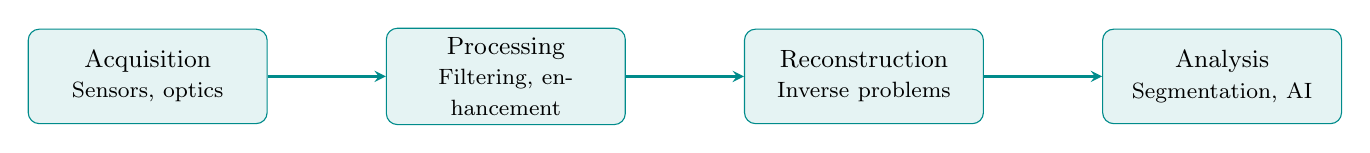
\begin{tikzpicture}[
        node distance=1.5cm,
        box/.style={rectangle, draw=imagingcyan, fill=imagingcyan!10, 
            text width=2.8cm, text centered, rounded corners, minimum height=1.2cm, font=\small},
        arrow/.style={thick,->,>=stealth,imagingcyan}
    ]
        \node[box] (acq) {Acquisition\\{\footnotesize Sensors, optics}};
        \node[box, right=of acq] (proc) {Processing\\{\footnotesize Filtering, enhancement}};
        \node[box, right=of proc] (recon) {Reconstruction\\{\footnotesize Inverse problems}};
        \node[box, right=of recon] (anal) {Analysis\\{\footnotesize Segmentation, AI}};
        
        \draw[arrow] (acq) -- (proc);
        \draw[arrow] (proc) -- (recon);
        \draw[arrow] (recon) -- (anal);
    \end{tikzpicture}
    \end{center}
    
    \vspace{0.3cm}
    \begin{columns}[T]
        \begin{column}{0.48\textwidth}
            \textbf{1. Acquisition:}
            \begin{itemize}
                \item Physical signal capture
                \item Sensor characteristics (noise, dynamic range)
                \item Sampling and discretization
            \end{itemize}
        \end{column}
        \begin{column}{0.48\textwidth}
            \textbf{2. Processing \& Analysis:}
            \begin{itemize}
                \item Noise reduction, artifact correction
                \item Feature extraction
                \item AI-based interpretation
            \end{itemize}
        \end{column}
    \end{columns}
\end{frame}

\begin{frame}{Y03: Understand digital image representation}
    \textbf{How are images represented digitally?}
    
    \vspace{0.3cm}
    \begin{columns}[T]
        \begin{column}{0.48\textwidth}
            \textbf{2D Images (Pixels):}
            \begin{itemize}
                \item Matrix of intensity values
                \item Grayscale: single channel (0--255)
                \item Color: RGB (3 channels)
                \item Resolution: pixels $\times$ pixels
            \end{itemize}
            
            \vspace{0.3cm}
            \textbf{3D Volumes (Voxels):}
            \begin{itemize}
                \item Stack of 2D slices
                \item Common in MRI, CT
                \item Isotropic vs. anisotropic
                \item Memory: $N^3$ voxels
            \end{itemize}
        \end{column}
        \begin{column}{0.48\textwidth}
            \textbf{Key Concepts:}
            \begin{itemize}
                \item \textbf{Spatial resolution:} Detail level
                \item \textbf{Intensity resolution:} Bit depth
                \item \textbf{Temporal resolution:} Frame rate
                \item \textbf{Spectral resolution:} Wavelengths
            \end{itemize}
            
            \vspace{0.3cm}
            \begin{block}{Medical Formats}
                \textbf{DICOM:} Standard for medical images\\
                \textbf{NIfTI:} Neuroimaging format\\
                \textbf{TIFF:} Microscopy standard
            \end{block}
        \end{column}
    \end{columns}
\end{frame}

\begin{frame}{Y04: Explain basic image processing operations}
    \textbf{Fundamental Image Processing Operations}
    
    \vspace{0.3cm}
    \begin{columns}[T]
        \begin{column}{0.32\textwidth}
            \textbf{Point Operations:}
            \begin{itemize}
                \item Brightness/contrast
                \item Histogram equalization
                \item Thresholding
                \item Intensity normalization
            \end{itemize}
        \end{column}
        \begin{column}{0.32\textwidth}
            \textbf{Spatial Filtering:}
            \begin{itemize}
                \item Smoothing (Gaussian)
                \item Sharpening (Laplacian)
                \item Edge detection (Sobel)
                \item Median filter (noise)
            \end{itemize}
        \end{column}
        \begin{column}{0.32\textwidth}
            \textbf{Morphological:}
            \begin{itemize}
                \item Erosion/dilation
                \item Opening/closing
                \item Hole filling
                \item Skeleton extraction
            \end{itemize}
        \end{column}
    \end{columns}
    
    \vspace{0.4cm}
    \begin{block}{Python Libraries}
        \textbf{scikit-image:} General image processing\\
        \textbf{OpenCV:} Computer vision\\
        \textbf{SimpleITK:} Medical image processing\\
        \textbf{scipy.ndimage:} N-dimensional images
    \end{block}
\end{frame}

% =====================================================================
% SECTION: Imaging Mass Cytometry
% =====================================================================
\section{Imaging Mass Cytometry}

\begin{frame}{Y05: Describe Imaging Mass Cytometry (IMC) and its applications}
    \textbf{What is Imaging Mass Cytometry?}
    
    \vspace{0.3cm}
    \begin{block}{Definition}
        IMC combines \textbf{immunohistochemistry} with \textbf{mass spectrometry} to simultaneously visualize 40+ protein markers in tissue sections at subcellular resolution.
    \end{block}
    
    \vspace{0.3cm}
    \begin{columns}[T]
        \begin{column}{0.48\textwidth}
            \textbf{How it works:}
            \begin{enumerate}
                \item Antibodies tagged with metal isotopes
                \item Laser ablates tissue pixel-by-pixel
                \item Mass spectrometer detects metals
                \item Reconstruct multiplexed images
            \end{enumerate}
        \end{column}
        \begin{column}{0.48\textwidth}
            \textbf{Applications:}
            \begin{itemize}
                \item Tumor microenvironment
                \item Immune cell profiling
                \item Spatial proteomics
                \item Drug response studies
                \item Biomarker discovery
            \end{itemize}
        \end{column}
    \end{columns}
    
    \vspace{0.3cm}
    \begin{alertblock}{Key Advantage}
        Unlike fluorescence microscopy (limited to 4--6 markers), IMC enables \textbf{highly multiplexed} analysis without spectral overlap.
    \end{alertblock}
\end{frame}

\begin{frame}{Y06: Explain how IMC enables multiplexed tissue analysis}
    \textbf{Multiplexed Analysis with IMC}
    
    \vspace{0.3cm}
    \begin{columns}[T]
        \begin{column}{0.48\textwidth}
            \textbf{Why multiplexing matters:}
            \begin{itemize}
                \item Single-marker analysis misses complexity
                \item Cell phenotypes require multiple markers
                \item Spatial context is crucial
                \item Understand cell--cell interactions
            \end{itemize}
            
            \vspace{0.3cm}
            \textbf{Typical panel design:}
            \begin{itemize}
                \item Structural markers (DNA, actin)
                \item Cell type markers (CD45, CD3, CD8)
                \item Functional markers (Ki67, PD-L1)
                \item Signaling markers (pSTAT3)
            \end{itemize}
        \end{column}
        \begin{column}{0.48\textwidth}
            \textbf{Analysis pipeline:}
            \begin{enumerate}
                \item Image preprocessing
                \item Cell segmentation
                \item Feature extraction
                \item Clustering / phenotyping
                \item Spatial analysis
            \end{enumerate}
            
            \vspace{0.3cm}
            \begin{block}{Tools}
                \textbf{steinbock:} IMC preprocessing\\
                \textbf{CellProfiler:} Cell segmentation\\
                \textbf{Squidpy:} Spatial analysis
            \end{block}
        \end{column}
    \end{columns}
\end{frame}

% =====================================================================
% SECTION: AI in Medical Image Analysis
% =====================================================================
\section{AI in Medical Image Analysis}

\begin{frame}{Y07: Understand the role of AI in medical image analysis}
    \textbf{AI is transforming medical imaging}
    
    \vspace{0.3cm}
    \begin{columns}[T]
        \begin{column}{0.48\textwidth}
            \textbf{Key AI Applications:}
            \begin{itemize}
                \item \textbf{Detection:} Find lesions, tumors
                \item \textbf{Segmentation:} Delineate structures
                \item \textbf{Classification:} Diagnose conditions
                \item \textbf{Quantification:} Measure volumes
                \item \textbf{Registration:} Align images
                \item \textbf{Reconstruction:} Enhance quality
            \end{itemize}
        \end{column}
        \begin{column}{0.48\textwidth}
            \textbf{Why deep learning excels:}
            \begin{itemize}
                \item Learns features automatically
                \item Handles high-dimensional data
                \item Generalizes across patients
                \item Processes images rapidly
            \end{itemize}
            
            \vspace{0.3cm}
            \begin{alertblock}{Clinical Impact}
                FDA has approved 500+ AI medical devices (2023), majority in radiology.
            \end{alertblock}
        \end{column}
    \end{columns}
\end{frame}

\begin{frame}{Y08: Describe image segmentation approaches}
    \textbf{Classical vs. Deep Learning Segmentation}
    
    \vspace{0.3cm}
    \begin{columns}[T]
        \begin{column}{0.48\textwidth}
            \textbf{Classical Methods:}
            \begin{itemize}
                \item Thresholding (Otsu)
                \item Region growing
                \item Watershed algorithm
                \item Active contours (snakes)
                \item Atlas-based methods
            \end{itemize}
            
            \vspace{0.2cm}
            \textbf{Pros:} Interpretable, no training\\
            \textbf{Cons:} Limited accuracy, tuning needed
        \end{column}
        \begin{column}{0.48\textwidth}
            \textbf{Deep Learning Methods:}
            \begin{itemize}
                \item U-Net (encoder-decoder)
                \item nnU-Net (self-configuring)
                \item Attention U-Net
                \item TransUNet (transformers)
                \item SAM (foundation model)
            \end{itemize}
            
            \vspace{0.2cm}
            \textbf{Pros:} State-of-the-art accuracy\\
            \textbf{Cons:} Requires labeled data
        \end{column}
    \end{columns}
    
    \vspace{0.3cm}
    \begin{block}{Best Practice}
        Use \textbf{nnU-Net} as a strong baseline -- it automatically adapts to your dataset and often achieves near-optimal performance.
    \end{block}
\end{frame}

\begin{frame}{Y09: Know about MedSAM}
    \textbf{Segment Anything in Medical Images (MedSAM)}
    
    \vspace{0.3cm}
    \begin{block}{What is MedSAM?}
        A \textbf{foundation model} for medical image segmentation, trained on 1.5 million image-mask pairs across 10 imaging modalities.
    \end{block}
    
    \vspace{0.3cm}
    \begin{columns}[T]
        \begin{column}{0.48\textwidth}
            \textbf{Key Features:}
            \begin{itemize}
                \item Based on Meta's SAM architecture
                \item Promptable segmentation
                \item Works across modalities
                \item Zero-shot generalization
                \item Interactive refinement
            \end{itemize}
        \end{column}
        \begin{column}{0.48\textwidth}
            \textbf{Modalities supported:}
            \begin{itemize}
                \item CT, MRI, X-ray
                \item Ultrasound, PET
                \item Dermoscopy, endoscopy
                \item Fundus, OCT
                \item Microscopy
            \end{itemize}
        \end{column}
    \end{columns}
    
    \vspace{0.3cm}
    \begin{alertblock}{Practical Use}
        MedSAM enables rapid annotation and can be fine-tuned for specific tasks.\\
        GitHub: \url{https://github.com/bowang-lab/MedSAM}
    \end{alertblock}
\end{frame}

% =====================================================================
% SECTION: Advanced Topics
% =====================================================================
\section{Advanced Topics}

\begin{frame}{Y10--Y11: LLMs and Multimodal Imaging}
    \begin{columns}[T]
        \begin{column}{0.48\textwidth}
            \textbf{Y10: LLMs in Medical Imaging}
            
            \vspace{0.2cm}
            \textbf{Emerging applications:}
            \begin{itemize}
                \item Report generation from images
                \item Visual question answering
                \item Image-text retrieval
                \item Clinical decision support
            \end{itemize}
            
            \vspace{0.2cm}
            \textbf{Key models:}
            \begin{itemize}
                \item GPT-4V for radiology
                \item Med-PaLM M (Google)
                \item LLaVA-Med
                \item BiomedCLIP
            \end{itemize}
        \end{column}
        \begin{column}{0.48\textwidth}
            \textbf{Y11: Multimodal Imaging}
            
            \vspace{0.2cm}
            \textbf{Combining modalities:}
            \begin{itemize}
                \item MRI + PET (anatomy + function)
                \item CT + SPECT (structure + perfusion)
                \item Histology + IMC (morphology + proteins)
            \end{itemize}
            
            \vspace{0.2cm}
            \textbf{Challenges:}
            \begin{itemize}
                \item Registration across modalities
                \item Different resolutions/scales
                \item Fusion strategies
                \item Interpretation complexity
            \end{itemize}
        \end{column}
    \end{columns}
    
    \vspace{0.3cm}
    \begin{block}{Future Direction}
        Foundation models trained on multimodal medical data will enable unified analysis across imaging, genomics, and clinical data.
    \end{block}
\end{frame}

% =====================================================================
% SUMMARY
% =====================================================================
\section*{Summary}

\begin{frame}{Summary: Computational Imaging}
    \textbf{Key Learning Points:}
    \begin{itemize}
        \item \textbf{Y01--Y04:} Fundamentals -- imaging pipeline, digital representation, processing
        \item \textbf{Y05--Y06:} Imaging Mass Cytometry -- multiplexed tissue analysis
        \item \textbf{Y07--Y09:} AI in imaging -- segmentation, MedSAM
        \item \textbf{Y10--Y11:} Advanced -- LLMs, multimodal imaging
    \end{itemize}
    
    \vspace{0.3cm}
    \begin{block}{Lab 4 Notebooks}
        \begin{tabular}{ll}
            00-test-installation & Verify environment \\
            01-imaging-intro & Basic imaging concepts \\
            02-mri-intro & MRI fundamentals \\
            03-imc-intro & Imaging Mass Cytometry \\
        \end{tabular}
    \end{block}
    
    \vspace{0.2cm}
    \begin{alertblock}{Connection to Individual Project}
        Computational imaging techniques can be applied to your individual project -- consider MRI analysis, segmentation, or IMC data.
    \end{alertblock}
\end{frame}

\end{document}

